\documentclass[12pt, letterpaper, twoside]{article}
\usepackage[utf8]{inputenc}
\usepackage[margin=1in]{geometry}
\usepackage{graphicx}
\usepackage{float}
\usepackage{color}
\usepackage{hyperref}
\usepackage{listings}
\usepackage{spverbatim}
\usepackage{fancyvrb}
\usepackage{fvextra}
\title{}
\author{}
%
\makeatletter
\setlength{\@fptop}{0pt}
\makeatother
\usepackage[figurename=Fig.]{caption}
%
\begin{document}
\maketitle

\section{Addressing the problems with distributed ledger technologies}\label{intro}
\begin{itemize}
	\item Definition of distributed system

	\item definition of ledger

	\item definition of distributed ledger

	\item implementations of distributed ledgers and their deployment
\end{itemize}

\subsection{Addressing the issues of distributed ledgers}\label{ledgerproblems}
security issues with distributed ledgers

definition of consensus and data consistency, probabilistic consensus + eventual data consistency

achieving consensus, attacchi alla data consistency, permissionless, sybils, attacchi di rete\\

nel capitolo seguente:

come bitcoin risolve le problematiche descritte dei distributed ledgers + definizione di pow + esempi di utilizzi di pow


\section{Introduction to Bitcoin}\label{sec:introbtc}
Bitcoin is a cryptocurrency and an electronic payment system built on a fully-decentralized peer-to-peer network.

It uses a permissionless blockchain as ledger and relies on \emph{Proof-of-Work} (PoW) based probabilistic consensus algorithm to achieve eventual data consistency~\cite{nakamoto}.

A Proof-of-work is a computational task given to peers, which solution is necessary to validate data appended to the blockchain. The high amount of time required to solve PoW puzzles makes attacks on the consensus algorithm infeasible, under the assumption that no user holds more than 50\% of the computing power on the network (see section~\ref{sec:securityintro}).

Moreover the structure of the blockchain, as shown in Section~\ref{fig:blockstruct}, makes tempering infeasible, thus ensuring the integrity of the data in blockchain.\\

In the following sections the reader will find an introduction to the Bitcoin network, where its main components and their function are analysed.


\subsection{An introductory example to Bitcoin usage}\label{sec:useexample}
A basic usage example, shown in Fig.~\ref{fig:basicexample}, is presented here to get the reader started with Bitcoin.

\begin{figure}[h!]
	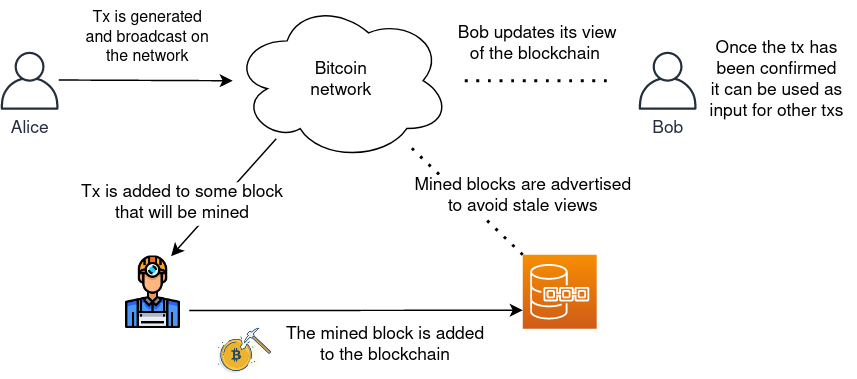
\includegraphics[width=.90\textwidth]{pict/basicexample.png}
	\centering
	\caption{Bitcoin introductory use case}
	\label{fig:basicexample}
\end{figure}

Let Alice and Bob be two Bitcoin users with a third-party wallet software. Each wallet is associated with a pair ECDSA keys used to identify users. The private key is used to sign issued transactions; instead, the public key is the Bitcoin address on which Bob can receive Bitcoins.

Suppose that Alice wants to transfer some amount of Bitcoins to Bob. Alice will generate a transaction in which she uses some set of unspent Bitcoins. The generated transaction will then be broadcast to the Bitcoin network.

A subset of the nodes, called miners, compete against one another in a parallel transaction confirmation process. Transactions are confirmed once they are included in a block added to the blockchain (\emph{mined} block).

To create a block, miners have to solve an exponentially difficult computational problem and therefore have to employ their computational power. The miner that first creates the new block earns Bitcoins, through a \emph{reward generating transaction} included in the block and the \emph{transaction fees} paid by the users whose transactions have been confirmed.

Once the transaction is included in the blockchain it is confirmed, thus the receiver will be able to spend again the transferred coins.

\subsection{Transaction structure}\label{sec:tx}
Transactions implement transfers and represent the entire set of coins available to users, and, when collected and ordered in the blockchain, its history. Hence, one can determine the balance of a certain wallet just by scanning the transactions on the blockchain~\cite{tschorsch-intro-survey}.

In Fig.~\ref{fig:tx} the reader can find the structure of a transaction, with its main fields.

\begin{figure}[h]
	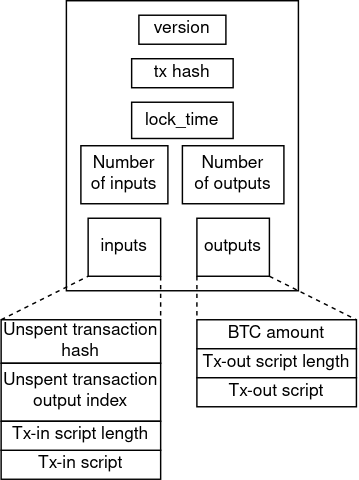
\includegraphics[width=.40\textwidth]{pict/txstruct.png}
	\centering
	\caption{Transaction structure}
	\label{fig:tx}
\end{figure}

In particular, the \texttt{lock\_time} field refers to the time or the blockchain height after which the transaction can be included in a block.

Transactions collect a set of \emph{inputs} and \emph{outputs}. Inputs are a collection of unspent coin sets, that are available to the user as previous transaction outputs or \textit{unspent transaction outputs} (UTXO). Outputs, instead, specify the number of coins to be transferred along with a receiver address.

Each input and output structure includes \emph{scripts}. These are sets of instructions, written in a Forth-like, stack-based language that describe the means to access the transferred coins. The script of a standard transaction includes a public key that, when hashed, yields a Bitcoin address, and a private key signature. The most common scripts on the market are \emph{Pay-to-PubKeyHash} (P2PKH) and \emph{Pay-to-ScriptHash} (P2SH).

Broadcasted transactions are verified before being added to a block and may be deemed invalid by honest miners and thus dropped. That might be the case for transactions that try to spend more than once the same set of coins or use invalid addresses. Nodes that broadcast invalid transactions may incur in bans if their behaviour is considered malicious.

\subsection{Block structure and blockchain}\label{sec:block}
The blockchain is a public distributed ledger, structured as an append-only linked list. It stores the entire transaction history of every peer in form of blocks.

In a block a set of transactions is bundled together and stored as a Merkle Tree, which ensures the data is unaltered and undamaged from the moment it is put into the block.

On top of that, each block contains the hash of the previous block in the blockchain and its own hash, thus preventing entirely block tempering for altering a transaction would result in mismatching hashes in the Merkle Tree, as well as in the stored block hash and in the hash in the next block in the blockchain.

Blocks have to be mined in order to be added to the blockchain. This means that the right \emph{nonce} needs to be found. The nonce is a varying value field that modifies the resulting hash of the block. A block is considered valid when a nonce such that the resulting hash is lower than a well-known \emph{target value} is found. That is equivalent to finding an hash that begins with $n$ zeroes.

Looking for the right nonce is exponential on $n$ number of zeroes.

The target value, and therefore the \emph{difficulty} of the computational task, is adjusted every 2016 blocks in order to keep the block generation and validation time around ten minutes.

Fig.~\ref{fig:blockstruct} shows the main fields stored in a block.

\begin{figure}[h]
	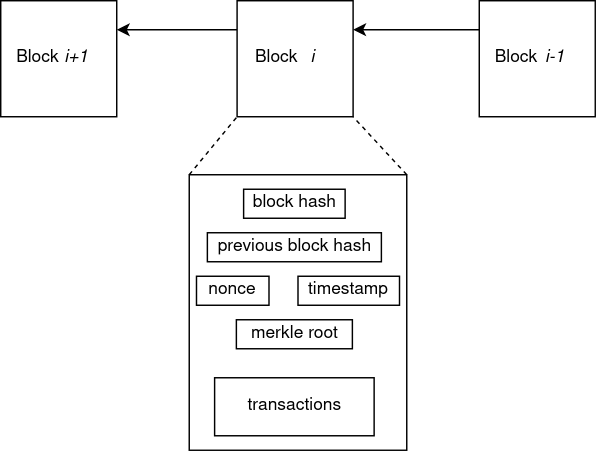
\includegraphics[width=.55\textwidth]{pict/blockstruct.png}
	\centering
	\caption{Block structure and blockchain}
	\label{fig:blockstruct}
\end{figure}

\subsection{Miners behaviour}\label{sec:miners}
The subset of peers that concurrently try to mine blocks by finding the right nonce are called miners, as described in Section~\ref{sec:block}. What motivates the miners to invest their computational power are mining rewards and transaction fees.

The mining reward is implemented as a transaction to the miner's wallet address that is included in the new block by the miner itself. Transaction fees are instead an amount of Bitcoins that the issuer of a transaction discretionally gives to the miners as an incentive for their work. Transactions with low transaction fees may incur in long processing times, since miners prioritize high rewards.\\

Transactions and blocks are gossiped through the network. Although each node has its own relay policy, it is in their interest, as honest miners, to get to know most of the pending transactions available for mining and to keep the view of the blockchain consistent at each node.

In particular, it is in the interest of miners to spread as fast as possible newly mined blocks in order to claim rewards and not waste time on stale views of the blockchain.

For the latter purpose, nodes need to keep their local blockchain view consistent with that of their neighbours. Nodes exchange \texttt{getblocks} messages to request \texttt{inv} messages which advertise local blocks. Missing blocks in a received \texttt{inv} message are retrieved with a \texttt{getdata} message~\cite{protocoldoc}. The described message exchange can be found in Fig.~\ref{fig:synch}.

Furthermore, \texttt{inv} messages are also gossiped when a node receives a new block. It is relevant to note that new blocks will be dropped by the receiving peers if any transaction is invalid or already spent. Nodes implicitly accept a block by starting to work on the next one, which contains the hash of last received valid block. 

\begin{figure}[h]
	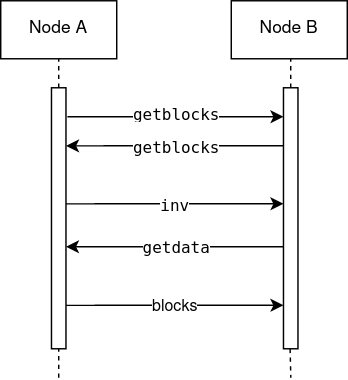
\includegraphics[width=.35\textwidth]{pict/blockchain-synch.png}
	\centering
	\caption{blockchain synch}
	\label{fig:synch}
\end{figure}

\subsection{Proof-of-Work and Consensus protocol}\label{sec:consensus}
In Bitcoin, as well as in other cryptocurrencies, the transaction verification process (mining) is distributed. The legitimacy of a transaction is verified by the majority of nodes before it is added to the public ledger, the blockchain.

These distributed environments are vulnerable to attacks in which a malicious user connects multiple fake replicas of himself to the network. If the number of fake attacking nodes exceeds that of the honest nodes, the attacker can forge any kind of data and validate it, thus appending it to the blockchain.

To avoid such scenarios, in order to append data to the blockchain, a Proof-of-Work is required. PoWs are cryptographic math puzzles that require scanning for a value, the nonce, which correct value attests that the node has put computational effort and time to verify the transaction(s). Mining is also described in Section~\ref{sec:useexample} and~\ref{sec:block}.

Thus, PoW discourages any kind of data forgery. Furthermore, tempering on the blockchain is impossible thanks to the definition of Merkle tree and blockchain, as described in Section~\ref{sec:block}. Bitcoin is therefore resistant both to tempering and forgery.

As mining is defined as a distributed process, and due to the lack of any central ledger, nodes may share inconsistent views of the blockchain. This is the case if relayed blocks are not delivered to some nodes or two or more nodes mine a new block approximately at the same time.

\emph{Forks} on the blockchain that are not maliciously engineered are solved by themselves by following a simple rule: only the longest branch of the blockchain is considered valid.

If two nodes are working on different branches of the same height, due to the random nature of mining, eventually one will release a new block before another. Hence its blockchain will be the longest and the only one considered correct.

To ensure that all nodes agree on the order of the entries of the blockchain, some simple rules are defined. More specifically, they state that:
\begin{enumerate}
	\item input and output values are rational
	\item transactions only spend unspent outputs
	\item all inputs being spent have valid signatures
	\item no transactions spend inputs with a \texttt{time\_lock} before the block in which they are confirmed
\end{enumerate} 
 
Bitcoin's PoW-based distributed consensus algorithm is defined as probabilistic since it guarantees eventual consistency. Furthermore it is generally considered robust and extremely scalable, as no authorization is required to join the network and mine.


\section{Bitcoin peer-to-peer protocol}\label{sec:netintro}

\subsection{Nodes and overlay topology}\label{sec:overlay}

bitcoin works on an overlay netowork

the overlay topology is unknown even though studied in the past

there are different kind of nodes that are part of the network, most of them do not take part in mining and stay behind NATs and dont accept incoming connections

Definition of full node

how many reachable nodes are out there https://bitnodes.io

In this work only full nodes are considered


\subsection{Connection and peer discovery}\label{sec:peerdisc}
In order to establish a connection two peers need to exchange version messages over an unencrypted TCP channel in a handshake fashion as shown in Fig.~\ref{fig:btcconn}. The node that first sends a \texttt{version} message establishes an \emph{outgoing connection}. The receiving node sets up an \emph{ingoing connection} instead. Once the handshake is completed the connection is fully set up.

\begin{figure}[h]
	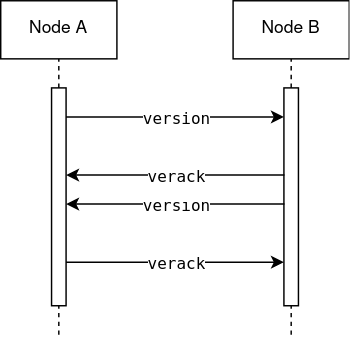
\includegraphics[width=.45\textwidth]{pict/BTCconnection.png}
	\centering
	\caption{Peers connection handshake}
	\label{fig:btcconn}
\end{figure}

Each node is capable to establish up to 8 outgoing connections and 117 ingoing connections, for a total of 125 connections. In order to keep its connections active, each peer sends a message to each neighbour at least once every thirty minutes. If more than ninety minutes pass without receiving anything from a neighbour, the connection is dropped.

Each node always tries to keep eight outgoing connections active, therefore, upon dropping an outgoing connection, a node tries to connect to another address in its peer cache.\\

Nodes on fresh bootstrap make use of hardcoded \emph{DNS seeds} as their first mean to discover other peers. DNS seed servers are maintained by community members and provide clients with a list of addresses that can be either dynamically gathered through a periodic scan of the network or manually updated by server administrators.

As a fallback option the user is able to specify through command line a list of addresses the client can connect to. Were both these two options to fail the client has a hardcoded list of peers it can directly connect to, though this is considered the last resort for bootstrapping peers.\\

Nodes at startup that were previously on the network shall first lookup peer names in their local address database, implemented as "peer.dat". The database contains the address of each peer the node has come to know during its lifetime in the network.

If the node has disconnected for a time too long, many of the addresses in the database may have become outdated or unreachable. A node that cannot connect to any address in the peer database, or has spent up to eleven seconds trying to connect unsuccessfully to at least one of the peers in the database, behaves as on fresh bootstrap and resolves to query a DNS first.

The use of a local address database, also called \emph{peer cache}, provides reconnecting peers a fully-decentralized way to join the network and is the first line of defence against \emph{fake bootstrap attacks}; the topic along with other security concerns is discussed in Chapter~\ref{sec:netsec}.\\

Peer discovery after the first connection of a node is carried on through the exchange of \texttt{addr} messages containing the address and port number of other peers in the network~\cite{protocoldoc},~\cite{devguidep2p}.

On connection set up the two nodes exchange \texttt{addr} messages, as shown in \emph{Fig.~\ref{fig:addr}}, providing each other with addresses from their local peer database.

On top of that, every twenty-four hours each node advertises itself on the network with an \texttt{addr} message containing only its own address.

\begin{figure}[h]
	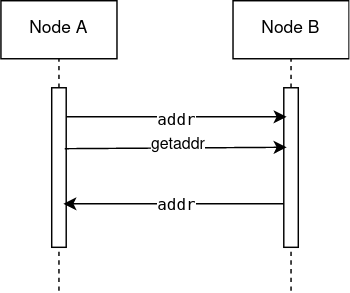
\includegraphics[width=.45\textwidth]{pict/BTCaddr.png}
	\centering
	\caption{Addresses exchange upon connection}
	\label{fig:addr}
\end{figure}

\texttt{addr} messages can contain at most one thousand addresses; additionally those containing ten or fewer addresses are relayed. This behaviour contributes to the gossiping of self-advertisement messages even though messages are relayed only to a small subset of neighbours, namely to a couple of peers.

\subsection{Peer database structure}\label{sec:cachestruct}
The local peer database or cache serves the purpose of storing the addresses a node has come to know from \texttt{addr} messages and DNS seeds. The database is constituted of the \texttt{new} and the \texttt{tried} tables.

The \texttt{tried} table contains addresses of peers with whom the node has successfully established a connection in the past. It consists of 64 buckets that can store up to 64 unique addresses. Buckets are selected through a hash on the IP address.

The \texttt{new} table contains the addresses the node has not connected to and is therefore larger: it has 256 buckets of 64 addresses each.

Peer caches have been widely implemented in distributed systems so far as they are a fast and fully-decentralized way to rejoin the network after a disconnection. They allow peer-to-peer systems to overcome major issues at bootstrap time, mainly related to the presence of a single point of failure, i.e. bootstrap servers. Furthermore, they are the most scalable and efficient solution when compared to other decentralized mechanisms such as \textit{address probing}~\cite{decentrbootstrapp2p}.

\subsection{Data dissemination}\label{sec:dissem}
definition of Gossip protocol, Diffusion,

btc nakatomo core client diffusion

dandelion

dandelion ++




\section{Bitcoin security concerns}\label{sec:securityintro}
\subsection{Common security threats on cryptocurrecies}
Bitcoin's decentralized, uncontrolled environment is open to a wide range of attacks, many of which are common threats for other cryptocurrencies as well. For this reason, the attacks described here can be carried out on other systems as well. These attacks have the same rationale, but different implementations.\\

Decentralized permissionless blockchains with PoW-based consensus algorithms are by definition vulnerable to \textit{51\%} or \textit{majority} attacks~\cite{nakamoto}. In these a user controls more than half of the computing power (often called \textit{hash rate}) available on the entire network~\cite{51atk}.

The attacker can thus subvert the consensus algorithm and validate harmful data, maliciously fork the blockchain or arbitrarily prevent blocks and transactions from verification.\\

Most of the malicious users that aim for a revenue from their attacks opt for \textit{double-spending} attacks. By definition, in double-spending attacks the same set of outputs is spent twice, hence the attacker gains Bitcoins or obtains resources from merchants for free.

Although proof-of-work consensus makes double-spending infeasible, since the transactions would not be validated, the attack can be still executed through other approaches. As a case in point, double-spending can be executed  if the attacker can successfully partition the network (see Section~\ref{sec:sybil}, or were other conditions to be met~\cite{doublespendfastpay}).\\

The way the correct state of the blockchain is elected, selecting the longest branch as the only valid, is exploitable for attacks that engineer block races.

In block races two or more peers spend computing power mining different forks of the same height. By definition of Bitcoin's consensus, there will be a point at which only one branch will be selected as valid and all the others will be discarded.

Block races can enable double-spending, as shown in Section~\ref{sec:sybil} and~\ref{sec:eclipse}, or mining attacks such as \textit{selfish mining}, where the malicious user holds private his mined blocks, thus forking the chain.

For the time the private chain of the attacker is longer that the public one, it can be released on the network, thus claiming the rewards for himself and wasting other miners' computing power~\cite{selfishmining}.\\

Since this chapter serves only introductory purposes, these are just a few attacks that can be driven onto Bitcoin. In the following sections there is more on network attacks, which are the focus of this thesis. The interested reader can find complete security overviews in the works of Conti et al., Saad et al. and Wang et al.~\cite{contiatksurvey},~\cite{saad2019attacksurface},~\cite{secpermissionlessblock}.

\subsection{Network security}\label{sec:netsec}
Attacks that exploit vulnerabilities in the design and implementation of the Bitcoin protocol and its peer-to-peer network fall under the category of network attacks.

Bitcoin is exposed to all the common threats that affect other peer-to-peer systems; these have been widely studied in the literature as in Touceda et al, 2012~\cite{toucedafakeboot}. The aim of this section is to understand how these attacks apply to Bitcoin and what are its defences\\

In network attacks. often the goal of the attacker is to alter the view of the network of a node, or group of nodes, by sending false network information or by connecting a large number of adversary-controlled peers to the victim, with the purpose of monopolizing its connections.

In this way network partitions, or other states in which the attacker can effectively control the data received by the victim, are created.

Nodes that become isolated from the network become vulnerable to \textit{N-confirmation double spending} or mining attacks, such as selfish mining or \textit{stubborn mining}~\cite{stubborn}. Furthermore 51\% attacks are easier to launch, since a part of the network computing power is cut off. 

For these reasons, network attacks are fundamental enablers for mining and spending attacks~\cite{dotan2020surveychallenges}.\\

In the following sections the reader can find both the attacks performed during the simulations reported in this thesis along with other network level attacks. These were added to better understand the mechanisms exploitable to carry out network attacks on cryptocurrencies.

\begin{figure}[h!]
	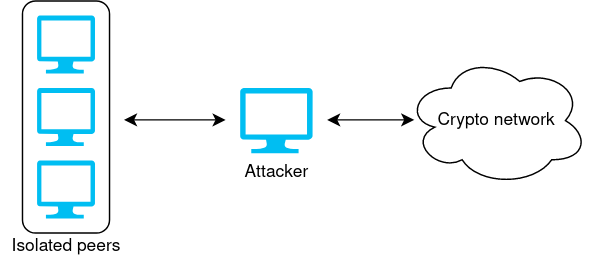
\includegraphics[width=.55\textwidth]{pict/network-partition.png}
	\centering
	\caption{Network partition}
	\label{fig:net-part}
\end{figure}


\subsubsection{Sybil attack}\label{sec:sybil}
In a Sybil attack a malicious user controls multiple identities on the network that can be either real machines or dummies, fake replicas of the attacker~\cite{douceur2002sybil}.

Such vector of attacks is applicable to any peer-to-peer system where users can create an arbitrary number of identities on the network for there is no node identification mechanism~\cite{kedziora-sybil-ledgers}. Thus, Bitcoin can suffer from such attacks.

Although the creation of fake identities cannot be exploited to carry out 51\% attacks, since they do not hold any computing power, they can still be used to spread forged information or to withhold blocks.

In the latter scenario, Sybil nodes, upon receiving a new block, send \texttt{inv} messages to their neighbours, but then leave unanswered the following \texttt{getdata} messages, thus delaying the propagation of blocks, as shown in \emph{Fig.~\ref{fig:sybil}}.

\begin{figure}[h!]
	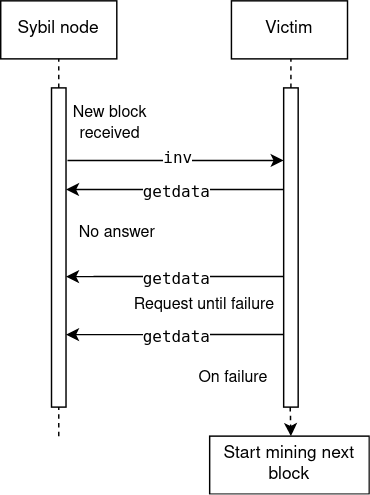
\includegraphics[width=.4\textwidth]{pict/sybil.png}
	\centering
	\caption{Sybil nodes behaviour during the attack}
	\label{fig:sybil}
\end{figure}

If the propagation is delayed long enough, the victim node could start mining the next block - in such scenarios a block race can be engineered. Block races occur whenever the blockchain is forked and different subsets of peers work on different branches of the chain.

Since only the longest chain stored among all peers is considered valid, all the other branches are dropped. The malicious user can exploit such forks to waste other peers' computing power or to perform double-spending~\cite{zhang-ds-sybil}. 

In the latter scenario, once the malicious user has successfully created a stale view of the blockchain in the victim, i.e. a fork, he releases two different transactions, Tx 1 and Tx 2, at the same time. Tx 1 is sent only to the victim node and Tx 2 is kept for its private chain, as shown in Fig.~\ref{fig:race1}.

In the meanwhile Sybil nodes hamper the growth both of the public and victim's blockchain by withholding blocks. As a result the attacker can mine the next block first and then release the private blockchain therefore invalidating the victim's blockchain, as shown in Fig.~\ref{fig:race2}.

\begin{figure}[h!]
	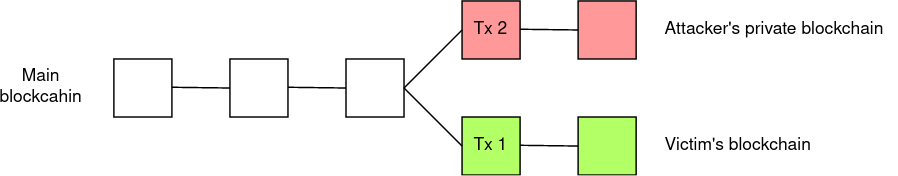
\includegraphics[width=.9\textwidth]{pict/blockrace1.png}
	\centering
	\caption{Block race for double-spending}
	\label{fig:race1}
\end{figure}

\begin{figure}[h!]
	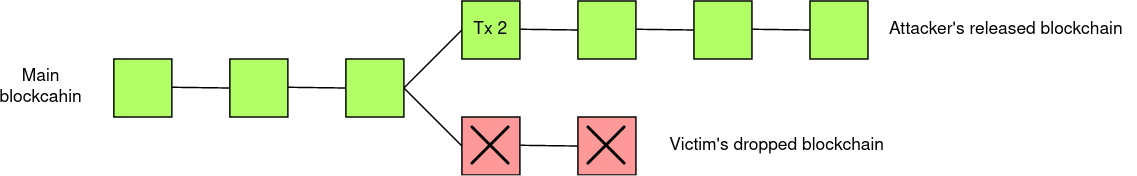
\includegraphics[width=.9\textwidth]{pict/blockrace2.png}
	\centering
	\caption{The attacker releases the longest chain}
	\label{fig:race2}
\end{figure}

Since Bitcoin requires no authentication or authorization to join the network, there will always be the possibility for adversaries to create Sybils. Nevertheless, countermeasures have been studied for different attacks based on Sybil attacks. For instance, setting a transaction block-confirmation timeout has been suggested by Zhang et al.~\cite{zhang-sybil-mitigations}.

Be that as it may, the implications of Sybil attacks are still a topic open to study. The interested reader can find more in the work of Iqbal et al.~\cite{iqbal-sybil}.

\subsubsection{Eclipse attack}\label{sec:eclipse}
The aim Eclipse attacks is to partition the network so that the attacker may be able to control all the data flowing between the two partitions.

In order to do that the malicious node, or a set malicious nodes, floods the victim with a multitude of incoming connections and feed it bogus network information, i.e. peer addresses controlled by the adversary, with \texttt{addr} exchanges, that will fill up their peer cache.

Upon restarting, with high probability the victim will form all of its eight outgoing connections with malicious IP addresses, thus finding itself isolated from the network.

Successful Eclipse attacks enable mining and spending attacks. Namely, eclipsing a subset of peers eliminates their mining power, hence making 51\% attacks easier. Selfish mining attacks can be carried out as well.

The attacker that successfully splits the network can also engineer block races to deliberately waste resources of other miners or attempt at double-spending attacks, as in Fig.~\ref{fig:race1} and Fig.~\ref{fig:race2}, described in Section~\ref{sec:sybil}.

Depending on the victim's policies, the malicious user can launch a \textit{0-confirmation double-spending attack}, that is for the case in which the merchant decides to release goods before the transaction is confirmed. As in the case of Sybil based double-spend, the attacker releases two transactions and keeps the victim's view of the blockchain stale, so that it would be dropped later (Fig.~\ref{fig:0confirm}).

Compared to the Sybil-based double-spending, Eclipse-based double-spending attacks of this kind have a greater chance of success, since they control all the victim's traffic and do not have to rely on delaying a block from spreading. Although the attacker needs to go through the partition set up first, whereas creating sybils is much easier.

\begin{figure}[h!]
	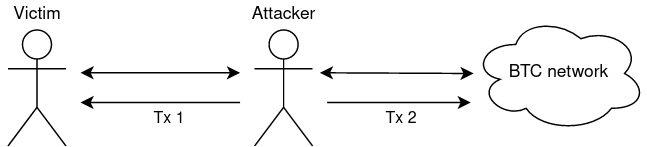
\includegraphics[width=.7\textwidth]{pict/0confirm-doublespend.png}
	\centering
	\caption{0-confirmation double-spend}
	\label{fig:0confirm}
\end{figure}

Were the victim to adopt a N-blocks confirmation policy for transactions, the attacker can still launch a \textit{N-confirmations double-spend} if it successfully eclipsed a subset of connected peers.

If that is the case, then the victims can be kept on an arbitrarily stale view of the blockchain and then be given one of the two transactions the attacker creates, while giving the other to the rest of the cryptocurrency network. After the eclipsed peers mine $N - 1$ blocks, the transaction is confirmed and the goods are exchanged. Thereafter, the obsolete branch of the blockchain known by the victims will be dropped once the attacker releases the up-to-date (and longer) version disseminated in the network (Fig.~\ref{fig:nconfirm} describes the process).

\begin{figure}[h!]
	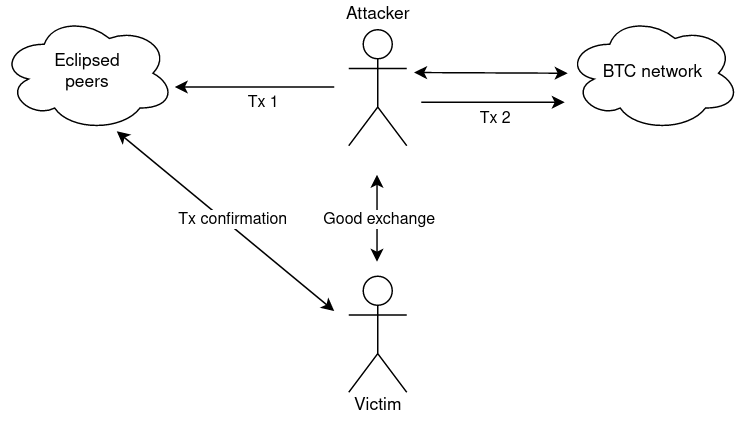
\includegraphics[width=.75\textwidth]{pict/nconfirm-doublespend.png}
	\centering
	\caption{N-confirmation double-spend}
	\label{fig:nconfirm}
\end{figure}

In 2015, Heilman et al. widely describe eclipse attacks and suggest many countermeasures to harden the network, a few of which were implemented in Bitcoin Core~\cite{eclipseatk}. As part of the adoption of these countermeasures, the number of buckets in \texttt{new} and \texttt{tried} has been increased, the addresses have become deterministically hashed to a single slot inside a bucket and the heavy bias towards addresses with fresher timestamps when choosing new connections has been removed.


\subsubsection{Fake bootstrapping attack}\label{sec:fakeboot}
Every peer-to-peer system needs some mean to let nodes join the network: in Bitcoin bootstrapping nodes need to rely on the information provided by some other peer in the network.

In a fake bootstrapping attack the peers contacted while a node is still initiating its connections, and hence its knowledge of the network, flood the bootstrapping peer with malicious addresses.

The results in Chapter~\ref{sec:res} show how feeding bogus information to a joining node can seriously influence its view of the network and lead to network partitions and peer eclipsing. This condition would also increase the efficacy of other network-level attacks, such as a DDoS, and the success rate of spending and mining attacks~\cite{eclipseatk}.\\

Prevention is done by ensuring a node can contact a trustworthy peer when joining the network. Peer caches and centralized bootstrap services serve this purpose, allowing joining nodes to make use of old neighbours while having central bootstrap servers as a fallback.

Other solutions have been implemented and tested over time, though their drawbacks usually exceed the benefits. As an example, randomly probing the address space, scouting for peers, decentralizes the bootstrap process and increases the variance of the network knowledge, but may not work if peers are behind NATs or firewalls and increases the latency for joining the network~\cite{decentrbootstrapp2p}~\cite{localityaware}.

In 2012,  Touceda et al. discuss fake bootstrapping along with other security threats in their survey~\cite{toucedafakeboot}.

Bitcoin employs many countermeasures, and overcomes other bootstrap issues, with its peer cache implementation mixed with external mechanisms: each node contacts its stored addresses for successive connections and aims to establish multiple outgoing connections, thus it does not rely on a single bootstrap node.

On top of that, DNS seeds provide a reliable external bootstrap service and the user is given the ability to manually insert addresses to connect to~\cite{mahmoud_netsec_boot}.


\subsubsection{DDoS attack}\label{sec:ddos}



\section{Enhancing the efficacy of Sybil attacks with fake bootstrapping}\label{sec:atk}
This study focuses on the influence that the dissemination of false network information has during the construction of the topology of the overlay network and how this enhances other network-level attacks.

The attack performed is a Sybil attack, described in section~\ref{sec:sybil}. Sybil nodes are used to increase the connections with honest nodes the attacker has, thus to have greater control on the data flowing in the network.  

In this study, Sybil nodes drop all transactions to and from a chosen victim to perform a denial-of-service. The reader can infer that the same results are applicable for block-withholding attacks.

As previously stated, malicious nodes disseminate bogus network information: they try to advertise as much as possible the addresses of other attackers through \texttt{addr} messages. Consequently, honest nodes are more likely to connect to malicious nodes.

The setting of the attack is during the construction of the overlay topology: at the start the graph is only a tree and many nodes are on fresh bootstrap. Nodes will all try to setup eight outgoing connections, emulating the behaviour of full nodes (Sec.~\ref{sec:peerdisc}). The way the graph forms is influenced by the network data advertised in this phase.

\subsection{Attack details}\label{sec:atkdetails}
The attack starts during the creation of the overlay topology, when nodes still have to setup the majority of their connections.

A group of at most $N$ nodes is on fresh bootstrap. The rest of the nodes are instead connected. The starting network graph is a tree, the choice comes from the need to have the sparsest graph possible.

In a series of rounds, nodes start to establish outgoing connections with addresses in their peer database. For honest nodes the upper bound on outgoing connections is eight, whereas there is no limitation for malicious nodes, that can therefore start connections with how many nodes they want. The choice is to make Sybil nodes prioritize connections with honest nodes, avoiding connections between each other.

Nodes on fresh bootstrap have to contact some DNS first. DNSs contain the data of a random subset of the nodes that were part of the network at the start. Their addresses will populate the bootstrapping node's peer database, that will then be able to connect to the network and start to establish more connections.

Network information is propagated through \texttt{addr} messages. These are exchanged upon establishing a connection. Bitcoin Core policy is to relay messages that contain at most ten addresses to a subset of neighbours~\cite{btccode}. For this reason, both attackers and honest nodes include in \texttt{addr} messages no more than ten addresses.

In the attack, honest nodes fill \texttt{addr} messages with a random subset of addresses in the peer database, malicious nodes advertise only attacking nodes' addresses instead (Fig.~\ref{fig:atkadrr}).

Moreover, Sybils do not relay incoming \texttt{addr} messages, thus hampering the propagation of honest nodes addresses. Attackers also work under the assumption that they share a common network knowledge, which means that once an attacker learns a new address, also all other attackers know it.

\begin{figure}[h!]
	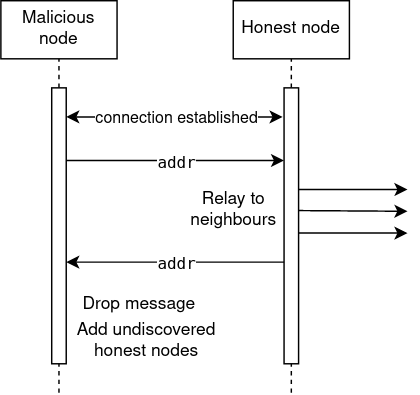
\includegraphics[width=.5\textwidth]{pict/atkaddr.png}
	\centering
	\caption{Peer discovery during the attack}
	\label{fig:atkadrr}
\end{figure}

On top of that, each node self-advertises its address with an \texttt{addr} message sent to its neighbours. Malicious nodes behave exactly as described before, dropping honest messages.

Once honest nodes cannot establish more connections, and the graph has become dense, the Sybil-based denial-of-service starts: Sybil nodes will drop all the transactions coming from the selected victim. 

The Sybil attack has two different setting that lead to different results. In the first one, Sybil nodes are all in network from the start.  In the second, all Sybil nodes are on fresh bootstrap. More can be found in Section~\ref{sec:res}.

\subsection{Metrics and performance evaluation}\label{sec:metrics}
The tests performed aim to understand how the aforementioned changes in the behaviour of nodes affect the effectiveness of the Sybil-based DoS attacks when adopting different dissemination protocols.

The coverage of a message is defined as the percentage of nodes reached in the network while adopting a certain dissemination protocol.

To evaluate the robustness of fixed probability broadcast and Dandelion ++, the coverage of victims' messages are estimated.

Coverage values of different protocols are carried out through different simulations, varying the number of attacking nodes and the underlying topology, as well as the number of attacking nodes.\\

Other metrics that are used to evaluate the efficacy of the new behaviour of Sybils are the average degree of malicious nodes and the average percentage of malicious neighbours for honest nodes.

These can describe how effectively Sybil nodes have connected to honest nodes, thus influencing the effectiveness of the subsequent Sybils attack.

Furthermore, the average percentage of Sybils in the peer cache is used to assess how well the bogus network information was disseminated.


\subsection{Software and implementation}\label{sec:softw}
The adopted simulator is LUNES-blockchain, a discrete event cryptocurrency-system simulator~\cite{lunes-paper}.

It consists of three main modules executed separately: topology creation, blockchain simulation and performance evaluation.

Topology creation is managed with the C library i-graph. Ideally, for each simulation a different set of graphs is generated.

Then the core simulation is run. Nodes mine blocks for the blockchain and exchange transactions and blocks with a previously specified dissemination protocol. The Sybil attack is carried out at this time.

At the end of the simulation, some scripts parse the data logged during the simulation and evaluate the robustness of the dissemination protocol.

The changes made to the behaviour of nodes apply only to the first part of the simulation: when nodes are still establishing outgoing connections. Only after this phase, the blockchain simulation is run and with the Sybil attack.

It is relevant to point out that the behaviour of nodes has been made as close as possible to that of Bitcoin full nodes.

The simulation proceeds as a series of epochs. In each epoch a different victim is randomly chosen among honest nodes, while the Sybil nodes are still the same from epoch to epoch.

All the tests are a collection of simulations. From a simulation to another the number of Sybil nodes is increased by some proportion of the total number of nodes in the network.

In the second attack scenario, when Sybils are all on fresh bootstrap, the number of total attackers in the network has been increased. Each run adds 100 Sybil nodes and the whole simulation is composed of 300 runs, for a total of 30000 attacking nodes.

On top of that, Sybil nodes join sequentially the network in the same epoch. This information is relevant to understand the results in Section~\ref{sec:external}.

\section{Results}\label{sec:res}
The results of the work of Serena et al. show how both Dandelion ++ and fixed probability gossip achieve high coverage (above $80\%$) even with an extremely high percentage of attackers in the network ($70\%$)\cite{lunes-dissemination}.

These results are confirmed with the following data obtained from new simulations shown in Fig..\\

Inserire grafico\\

Changing the behaviour of Sybil nodes to disseminate bogus network information, as described in Section~\ref{sec:atkdetails}, yields the results shown in Fig.~\ref{fig:in-cov}.

The outcome is similar for every protocol: coverage drops steeply for each of them, thus confirming the efficacy of the new behaviour.

Despite achieving the best coverage in previous results, even Dandelion ++ seems ineffective.\\

\begin{figure}[h!]
	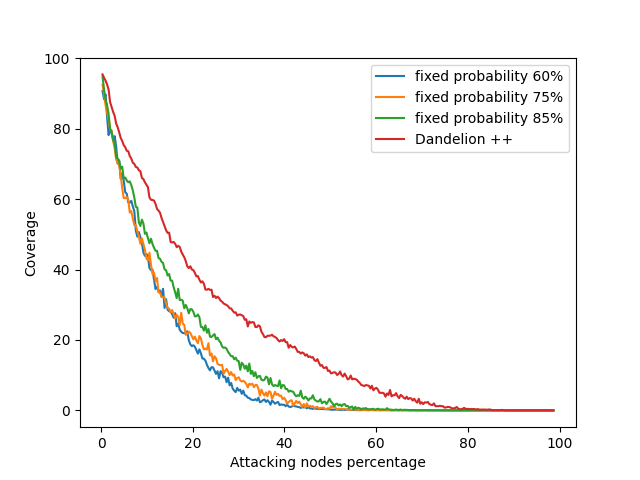
\includegraphics[width=.7\textwidth]{pict/results/in-cov.png}
	\centering 
	\caption{Coverage results}
	\label{fig:in-cov}
\end{figure}

The following metrics are reported in order to study the topology of the new network and to assess how well the new behaviour of malicious nodes has worked.

The average degree of honest nodes reveals that each node is highly connected and has on average an higher degree than those in the results of Serena et al. (Fig...). \\

\begin{figure}[h!]
	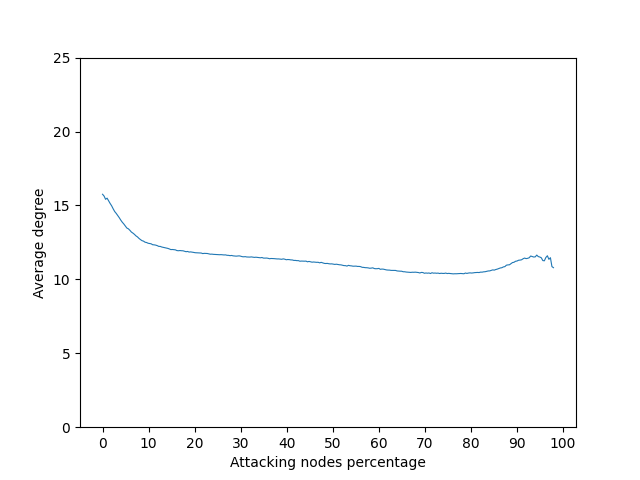
\includegraphics[width=.7\textwidth]{pict/results/in-hon-avg-neigh.png}
	\centering
	\caption{Average degree of honest nodes}
	\label{fig:degreehon}
\end{figure}

The average percentage of malicious neighbours is shown in Fig.~\ref{fig:avgatk}. It is fundamental to evaluate the efficacy of the new Sybils behaviour, as the closer they get to eclipse honest nodes the higher the chance of carrying out a block-withholding attack would be.\\

\begin{figure}[h!]
	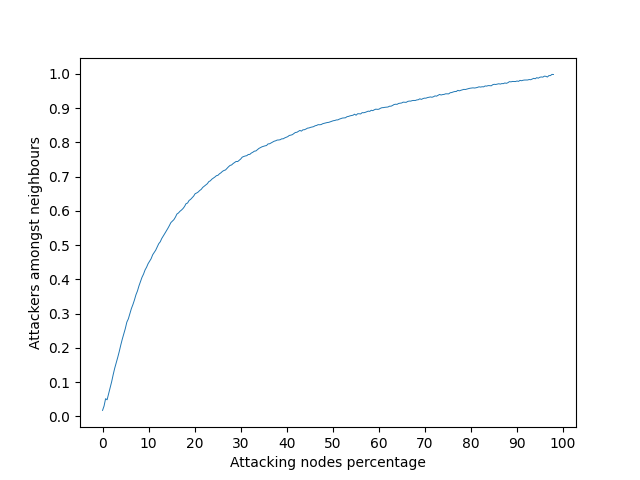
\includegraphics[width=.7\textwidth]{pict/results/in-hon-avg-neigh-atk.png}
	\centering
	\caption{Average percentage of Sybils among neighbours}
	\label{fig:avgatk}
\end{figure}

Furthermore, the reader can see how well false network information was spread in the graph shown in Fig.~\ref{fig:avgatk-known}, as it depicts the percentage of malicious nodes in the peer cache of honest nodes.

The data can also be interpreted as the probability of a node connecting to a Sybil, since new connections are chosen uniformly at random from the cache.\\

\begin{figure}[h!]
	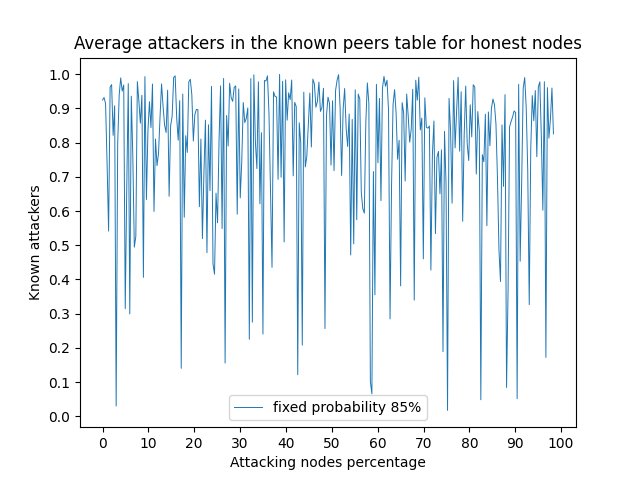
\includegraphics[width=.7\textwidth]{pict/results/in-hon-avg-known-atk.png}
	\centering
	\caption{Average percentage of Sybils in the peer cache}
	\label{fig:avgatk-known}
\end{figure}

The average degree of malicious nodes (Fig.~\ref{fig:in-atk-degree}) shows Sybils far more connected than honest nodes, especially when they fewer. This is due to the lack of an upper bound on outgoing connections.

The descending trend of the degree is due to malicious nodes avoiding making connections between themselves. When the number of attacking nodes increases, that of honest nodes decreases proportionally, thus leaving fewer nodes to connect to.

With a samples of the degree distribution, Fig.~\ref{fig:incluster}, it is possible to understand how the topology of the underlying network was influenced. 

Where there is a low percentage of Sybils in the network malicious nodes tend to have on average an extremely high degree.

As the percentage increases the tendency to create clusters emerges: some Sybils reach extremely high degrees, whilst others are left poorly connected.\\
\begin{figure}[h!]
	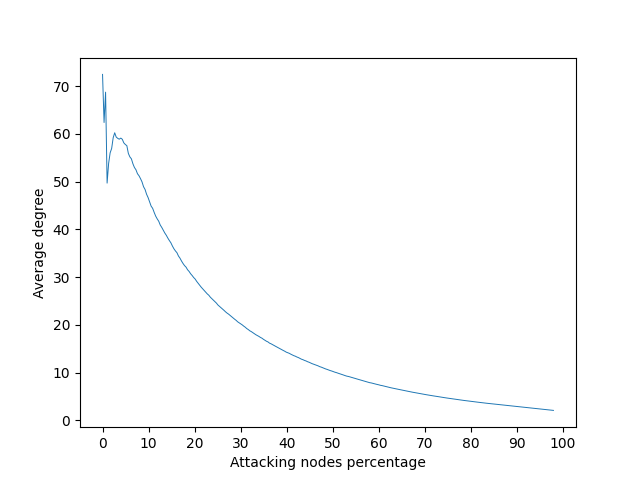
\includegraphics[width=.7\textwidth]{pict/results/in-atk-avg-degree.png}
	\centering
	\caption{Average degree of Sybil nodes}
	\label{fig:in-atk-degree}
\end{figure}

\begin{figure}[h!]
	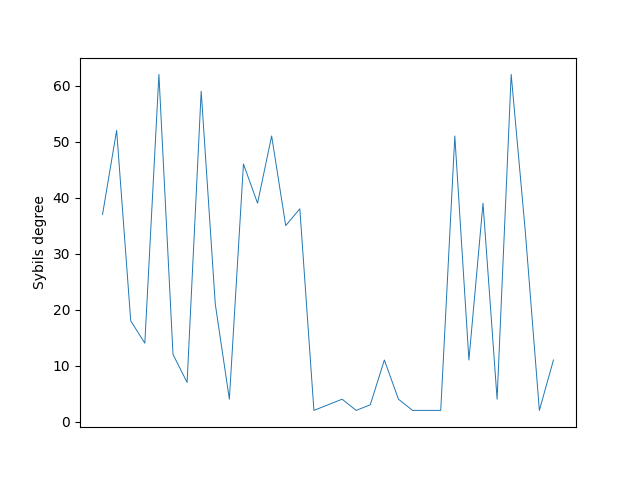
\includegraphics[width=.7\textwidth]{pict/results/in-cluster.png}
	\centering
	\caption{Sample of degree distribution of Sybil nodes}
	\label{fig:incluster}
\end{figure}

Also DNSs their role to determine the efficacy of the attack. The percentage of malicious addresses in their peer lists directly influence  the chance of a node on fresh bootstrap connecting to a malicious node first. Fig.~\ref{fig:dns} shows a steady increase in the percentage of malicious addresses.

\begin{figure}[h!]
	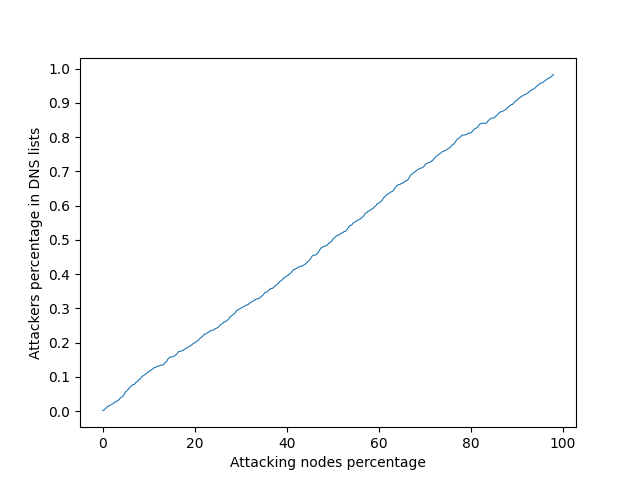
\includegraphics[width=.7\textwidth]{pict/results/in-dns.png}
	\centering
	\caption{Percentage of Sybils in the DNSs}
	\label{fig:dns}
\end{figure}

\subsection{Alternative attack scenario}\label{sec:external}
In the second attack scenario all malicious nodes are on fresh bootstrap and have to join the network while it is still forming. The number of attacking nodes in these simulations has been increased up to 30000. A total of 300 simulations are run, 100 attacking nodes are added at each.\\

The attack does not achieve any results in this scenario, as shown by the coverage in Fig.~\ref{fig:ext-cov}. The network is thus resistant to such Sybil attack.\\

\begin{figure}[h!]
	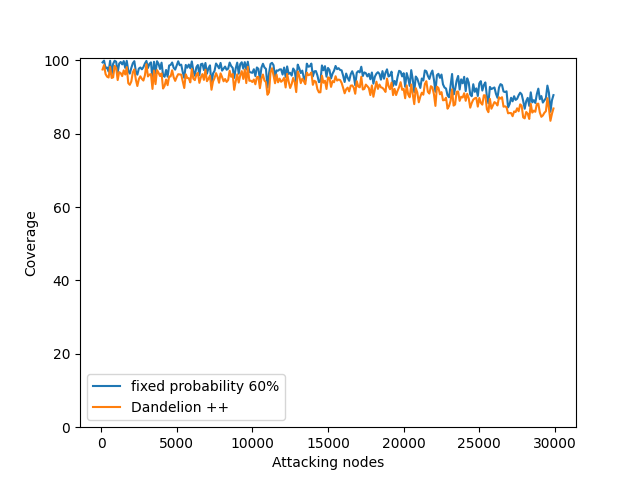
\includegraphics[width=.7\textwidth]{pict/results/ext-cov.png}
	\centering
	\caption{Coverage with Sybils on fresh bootstrap (second scenario)}
	\label{fig:ext-cov}
\end{figure}



Also the the changes in the behaviour of Sybils have been ineffective, since rate of malicious neighbours is significantly lower (Fig.~\ref{fig:ex-atk-neigh}).\\

\begin{figure}[h!]
	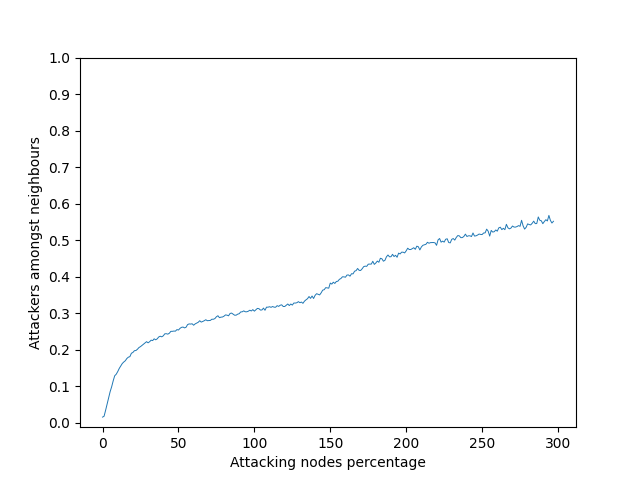
\includegraphics[width=.7\textwidth]{pict/results/ext-hon-atk-neigh.png}
	\centering
	\caption{Percentage of Sybil neighbours in the second attack scenario}
	\label{fig:ex-atk-neigh}
\end{figure}

Despite that, Sybils still managed to disseminate malicious addresses well, although achieving results worse than those in the previous setting (Fig.~\ref{fig:ex-atk-known}).\\

\begin{figure}[h!]
	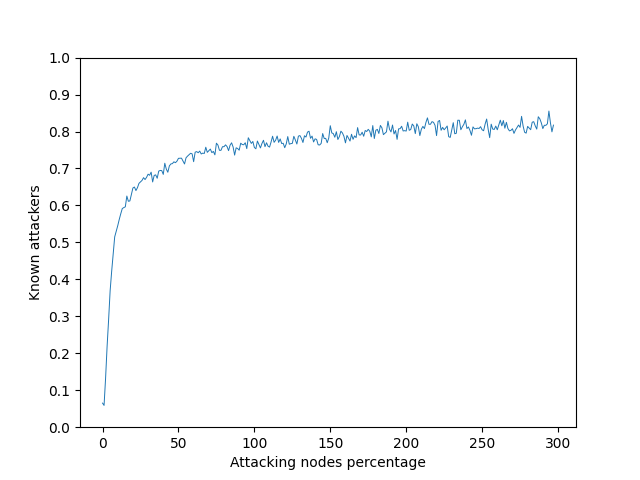
\includegraphics[width=.7\textwidth]{pict/results/ex-hon-atk-known.png}
	\centering
	\caption{Percentage of Sybils in the peer cache}
	\label{fig:ex-atk-known}
\end{figure}

Also the shape of the graph has changed. Sybils are less connected and face the same downward trend in the average degree, Fig.~\ref{fig:ex-atk-degree}, as a result of the increasing number of attackers.

Moreover, by looking at a sample degree distribution, Fig.~\ref{fig:dd}, the reader can see that only the Sybils that connect first (they connect sequentially Sec.~\ref{sec:softw}) are able to establish more connections, while the others are left in sparser areas of the graph.\\

\begin{figure}[h!]
	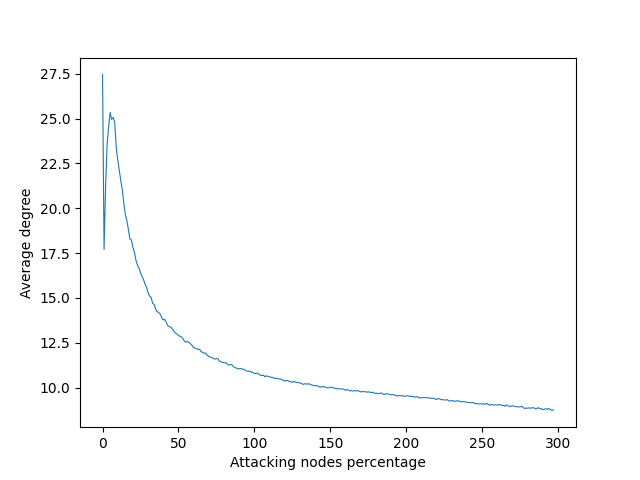
\includegraphics[width=.7\textwidth]{pict/results/ex-atk-avg-degree.png}
	\centering
	\caption{Sybils average degree in the second attack scenario}
	\label{fig:ex-atk-degree}
\end{figure}

\begin{figure}[h!]
	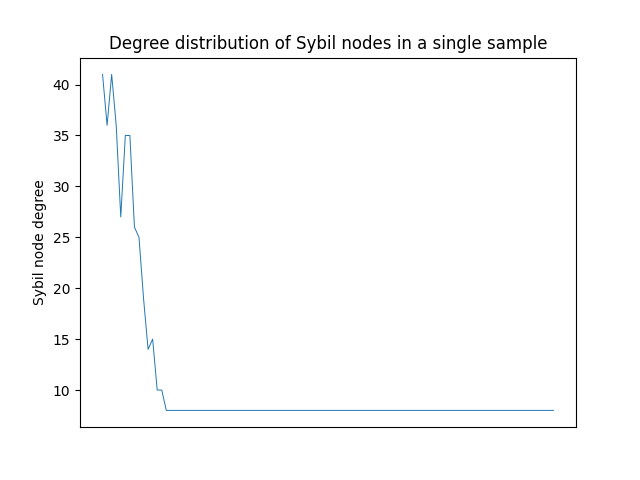
\includegraphics[width=.7\textwidth]{pict/results/ex-atk-dd.png}
	\centering
	\caption{Sample of Sybils degree distribution in the second attack scenario}
	\label{fig:dd}
\end{figure}

In this scenario DNS peer lists did not have any attacker, since they cannot contain nodes on fresh bootstrap.

\section{Conclusions}\label{sec:concl}
The way malicious nodes disseminate bogus network information makes the attack resemble fake bootstrapping. In particular, the adversary exploits \texttt{addr} messages exchanges and their relay policy to extensively disperse false network information. 

The efficacy of the strategy has been proven high, as with just 10\% of the identities on the network the adversary can fill peer caches with malicious addresses.

Furthermore, the Sybil attack executed on the new overlay network is substantially more powerful, as it makes coverage drop steeply with less malicious nodes involved in the attack.

It is necessary to point out that the new Sybil attack achieves high efficacy despite working with a network far more dense than the one in the results of Serena et al. Their work assessed the importance of an highly connected graphs as a direct countermeasure to Sybil attacks of this kind.

Therefore, the results obtained imply an increased feasibility of the attack, since the adversary needs to control fewer identities to disrupt honest activities. With just the 20\% of the nodes it is possible to make coverage drop below 40\%.\\

Nonetheless, the setting of the attack is ideal and cannot be compared to that of a real network. The positive outcome is influenced by the increased capability to spread network information during the time the graph topology is still forming.

Under no circumstances the real Bitcoin network could undergo such process. For this reason the attack has been carried out on a second scenario where all the malicious nodes are on fresh bootstrap.

The results in Fig.~\ref{fig:ext-cov} show how the attack was utterly ineffective even though the network was still being built at the time the Sybils started to join.
 
Furthermore, also the new behaviiour of Sybils did not work, since the average percentage of attacking neighbours (Fig.~\ref{fig:ex-atk-neigh}) is significantly lower.

Despite that, there is no gap that big in the rate of Sybils in the peer cache (Fig.~\ref{fig:ex-atk-known}) between the two attack scenarios, thus stating the attackers could still disseminate rather well their addresses.

This means that the positive outcome of the attack in the first scenario was influenced by two factors: the presence of Sybils in the DNS lists and the time at which malicious addresses start to be disseminated.

Although the first factor has been surely influential in later stages of the simulation, when the number of attackers increased, it is required to assess the importance of the latter.

The data in Fig.~\ref{fig:beginning} shows the percentage of malicious addresses in peer caches before bootstrapping nodes start to join.

\begin{figure}[h!]
	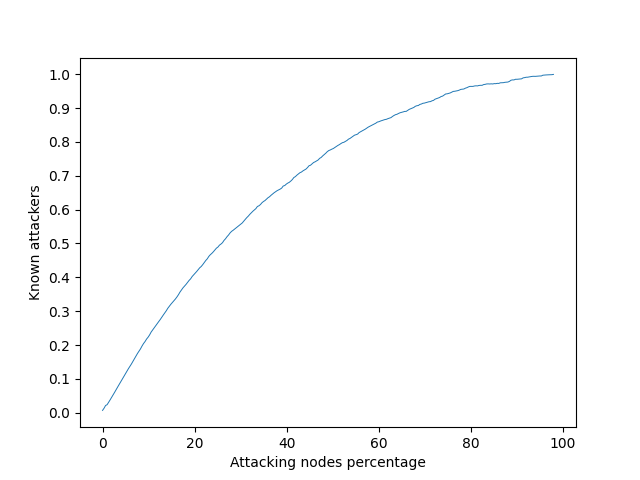
\includegraphics[width=.7\textwidth]{pict/results/in-atkknown-beginning.png}
	\centering
	\caption{Percentage of Sybils in the peer cache at the beginning of the graph construction}
	\label{fig:beginning}
\end{figure}

...

On the other hand, in future work it is possibile to have a graph already formed and try to mix it with an eclipse attack described by heilman et al 2015

Nonetheless, steep falls attack doesnt work properly

Moreover, the second attack scenario has demonstrated that











\bibliographystyle{plain}
\bibliography{bib.bib}

\end{document}